%%%%%%%%%%%%%%%%%%%%%%%%%%%%%%%%%%%%%%%%%%%%%%%%%%%%%%%%%%%%%%%%%%%%%%%%%%%%%%%%%%%%%%%%%%

% DIT MATERIAAL VERTROK VAN DE OPEN-SOURCE CURSUS VEELTERMEN VAN KOEN DE NAEGHEL         
% GEKOPIEËRD OP 24 MAART 2025                                                            
% ORIGINEEL BESCHIKBAAR VIA https://www.koendenaeghel.be/opensource.htm         

%%%%%%%%%%%%%%%%%%%%%%%%%%%%%%%%%%%%%%%%%%%%%%%%%%%%%%%%%%%%%%%%%%%%%%%%%%%%%%%%%%%%%%%%%%



\documentclass{ximera}
\input{../preamble}
\input{../preamblekdn}

\addPrintStyle{..}
\begin{document}
	\author{Koen de Naeghel - Wiskunde Op Maat}
	\xmtitle{Schema van de staartdeling}{}
    \xmsource




In de lagere school heb je geleerd hoe je een deling van twee gehele getallen kan uitvoeren met behulp van het schema van de staartdeling. De staartdeling is een voorbeeld van wat we een \textit{ algoritme} noemen: een eindige reeks instructies om vanuit een gegeven begintoestand een probleem op te lossen of een taak uit te voeren. Zo is ook een keukenrecept een  voorbeeld van een aloritme. De fundamentele vraag welke problemen met een algoritme kunnen opgelost worden, werd in 1937 opgelost door Alan Turing. Zijn werk lag aan de basis van een van de grootste uitvindingen ooit: de computer. De deling van \(239\) door \(5\) als quotiënt \(47\) en rest \(4\). Dat resultaat kun je schrijven als \(239 = 5 \cdot 47 + 4\). Kenmerkend is dat de rest kleiner is dan (de absolute waarde van) de deler. 
	
Hieronder leer je om een deling van veeltermen -met het algoritme van de staartdeling- op een gelijkaardige manier uit te voeren.
	
\begin{algorithm}(staartdeling)
	We hernemen het voorbeeld \(A(x) = 14x^2+17x+5\) en \(B(x) = 2x+1\). Om na te gaan dat \(B(x)\) een deler van \(A(x)\) is en om tegelijk ook het quotiënt te vinden, kan je stapsgewijs \textit{ de veelterm \(B(x)\) forceren in de veelterm \(A(x)\)}. Dat gaat als volgt:
	\begin{align*}
	14x^2 + 17x + 5 
	& = \red{7x} \cdot (2x+1) \blue{- 7x} + 17x + 5 \\
	& = \red{7x} \cdot (2x+1) + 10x + 5 \\
	& = \red{7x} \cdot (2x+1) + \red{5} \cdot (2x+1) \blue{- 5} + 5 \\
	& = \red{7x} \cdot (2x+1) + \red{5} \cdot (2x+1) \\
	& = (2x+1)\cdot(\red{7x + 5}).
	\end{align*}
	
	
	
	Het vele schrijfwerk kan ingekort worden door het onderstaande \textit{ schema van de staartdeling}, ook wel \textit{ lange deling} genoemd. Hierin herken je de stappen die hierboven werden uitgevoerd. 

	\tikzit{
	\(
	\begin{array}{l|l}
	& 2x+1 \\
	\cline{2-2}
	\vrule height 1.2em width 0pt
	& \red{7x+5} \\[-0.96cm]
	\stackunder[0.05cm]{%
	  \stackon[0pt]{14x^2+17x+5}{}%
	}{%
	  \Shortstack[r]{
		{14x^2+\mph{1}\blue{7x}\mph{+5}}
		{\staartmin \staartstreep{14x^2+\mph{1}7x} \staartphstreep{+50}}
		{10x+5}
		{10x+\blue{5}} 
		{\staartmin \staartstreep{10x+5}}
		{0}
	}
	}  
	\end{array}
	\)
	}

	Hieruit besluiten we dat \(B(x) = 2x+1\) een deler is van \(A(x) = 14x^2+17x+5\), want er bestaat een veelterm \(Q(x)\) waarvoor \(A(x) = B(x) \cdot Q(x)\), namelijk \(Q(x) = 7x+5\). In symbolen:
	\[
	\underbrace{14x^2+17x+5}_{A(x)} = \underbrace{(2x+1)}_{B(x)}\cdot\underbrace{(7x + 5)}_{Q(x)}.
	\]

	Ook in het geval een veelterm \(A(x)\) niet deelbaar is door een veelterm \(B(x)\), kan je te werk gaan zoals hierboven. Het \textit{ forceren van de veelterm \(B(x)\) in de veelterm \(A(x)\)} verloopt dan als volgt:
	\begin{align*}
	2x^3 + 3x^2 - 1 
	& = \red{2x} \cdot (x^2+3x) \blue{- 6x^2} + 3x^2 - 1 \\
	& = \red{2x} \cdot (x^2+3x) - 3x^2 - 1 \\
	& = \red{2x} \cdot (x^2+3x) \red{- 3} \cdot (x^2+3x) \blue{+ 9x} - 1  \\
	& = (x^2+3x) \cdot (\red{2x - 3}) + 9x - 1.
	\end{align*}
	Het bijbehorende schema van de staartdeling vergt opnieuw minder schrijfwerk. 

	\tikzit{
	\(
	\begin{array}{l|l}
	& x^2+3x \\
	\cline{2-2}
	\vrule height 1.2em width 0pt
	& \red{2x-3} \\[-0.96cm]
	\stackunder[0.05cm]{%
	  \stackon[0pt]{2x^3+3x^2-1\mph{x-1}}{}%
	}{%
	  \Shortstack[r]{
		{2x^3 \blue{+6x^2}\mph{-9x-1}} 
		{\staartmin \staartstreep{2x^3+6x^2} \staartphstreep{-9x-10}}
		{-3x^2-1\mph{x-1}} 
		{-3x^2 \blue{-9x}\mph{-1}} 
		{\staartmin \staartstreep{-3x^2-9x} \staartphstreep{-10}}
		{9x-1}
	}
	}  
	\end{array}
	\)
	}

	In dit geval stopt de procedure bij een \textit{restveelterm} (kortweg \textit{ rest}) \(R(x)\) die verschillend is van nul. Kenmerkend is dat de graad van die rest kleiner is dan de graad van \(B(x)\). Uit het bovenstaande schema van de staartdeling mogen we dus besluiten dat
	\[
	\underbrace{2x^3+3x^2-1}_{A(x)} = \underbrace{(x^2+3x)}_{B(x)}\cdot\underbrace{(2x - 3)}_{Q(x)} \,\, + \,\, \underbrace{9x - 1}_{R(x)} \quad \text{ waarbij } \quad \gr R(x) < \gr B(x).
	\]

	\end{algorithm} 
	
	In het vervolg wordt meestel enkel het schema van de staartdeling opgeschreven. Onthoud wel waar die staartdeling vandaan komt: het is een kortere schrijfwijze voor het \textit{ forceren van een veelterm \(B(x)\) in een veelterm \(A(x)\)}, de langere werkwijze die we hierboven twee keer uitgeschreven hebben. Enerzijds komt die lange werkwijze later nog aan bod in bewijzen van eigenschappen. Anderzijds komt ze ook nog van pas bij het oplossen van sommige oefeningen, net zoals dat bij de \textit{methode van de onbepaalde coëfficiënten} het geval is.
	
	


	Het volgende voorbeelden gaan voor twee gegeven veeltermen deelbaarheid met de staartdeling na: 


	\begin{example} 
	Beschouw de veeltermen \(A(x) = 6x^3 + 19x^2 + 8x - 5\) en \(B(x) = 2x+5\). We gaan met behulp van het schema van de staartdeling na of \(A(x)\) deelbaar is door \(B(x)\). 
	
	\tikzit{
	\(
	\begin{array}{l|l}
	& 2x+5 \\
	\cline{2-2}
	\vrule height 1.2em width 0pt
	& 3x^2+2x-1 \\[-0.96cm]
	\stackunder[0.05cm]{%
	  \stackon[0pt]{6x^3+19x^2+\mph{0}8x-5}{}%
	}{%
	  \Shortstack[r]{
		{6x^3+15x^2\mph{+08x-5}} 
		{\staartmin \staartstreep{6x^3+15x^2} \staartphstreep{+10x-50}}
		{4x^2+\mph{0}8x-5} 
		{4x^2+10x\mph{-5}} 
		{\staartmin \staartstreep{4x^2+10x-5}}
		{-2x-5}
		{-2x-5}
		{\staartmin \staartstreep{-2x-5}}
		{0}
	}
	}  
	\end{array}
	\)
	}
	
	Uit dit schema volgt het verband tussen deeltal, deler, quotiënt en rest:
	\[
	\underbrace{6x^3 + 19x^2 + 8x - 5}_{A(x)} = \underbrace{(2x+5)}_{B(x)}\cdot\underbrace{(3x^2+2x-1)}_{Q(x)} \,\, + \,\, \underbrace{0}_{R(x)} 
	\]
	waaruit we besluiten dat \(A(x)\) deelbaar is door \(B(x)\).
	\end{example} 


Deelbaarheid voor veeltermen met parameters werd voor de staartdeling al nagegaan met de \textit{methode van de onbepaalde coëfficiënten}. Het algoritme van de staartdeling werkt echter altijd. Ook in dit geval kan het ook hier -al is het niet het meest efficiënt-  toegepast worden: 

\begin{example} 
Gegeven is de veelterm \(A(x) = x^3 + ax^2 - 9x + b\) waarbij \(a,b \in \R\). We bepalen de waarde(n) van de parameters \(a\) en \(b\) waarvoor \(A(x)\) deelbaar is door \((x+1)^2\). Dat kunnen we doen met behulp van het schema van de staartdeling:
\tikzit{
\(
\begin{array}{l|l}
& x^2+2x+1 \\
\cline{2-2}
\vrule height 1.2em width 0pt
& x+a-2 \\[-0.96cm]
\stackunder[0.05cm]{%
	\stackon[0pt]{x^3 + ax^2 - 9x + b}{}%
}{%
	\Shortstack[r]{
	{x^3 + 2x^2 + x\mph{9+b}} 
	{\staartmin \staartstreep{(a-2)x^2-10x+b}}
	{(a-2)x^2-10x+b} 
	{(a-2)x^2 + (2a-4)x + a-2} 
	{\staartmin \staartstreep{(a-2)x^2 + (2a-4)x + a-2}}
	{(-2a-6)x+b-a+2}
}
}  
\end{array}
\)
}

waaruit volgt dat  
\begin{align*}
(x+1)^2 \mid A(x) \quad 
& \Leftrightarrow \quad (-2a-6)x+b-a+2 = 0x + 0 \\
& \Leftrightarrow \quad
\left\{ 
\begin{aligned}
-2a-6 & = 0 \\
b-a+2 & = 0 
\end{aligned}
\right. \\ 
& \Leftrightarrow \quad
\left\{ 
\begin{aligned}
a & = -3 \\
b & = -5. 
\end{aligned}
\right.
\end{align*} 

Een andere manier om \(a\) en \(b\) te bepalen is door middel van de methode van de onbepaalde coëfficiënten. Dat blijkt efficiënter te zijn dan het schema van de staartdeling, omdat je heel wat minder rekenwerk moet uitvoeren: het quotiënt van de opgaande deling van \(A(x)\) door \((x+1)^2 = x^2 + 2x + 1\) heeft graad \(1\) en vergelijken van hoogstegraadsterm en constante term in linker- en rechterlid geeft meteen:

\begin{align*}
x^3 + ax^2 - 9x + b 
& = (x^2 + 2x + 1)(x + b) \\
& = x^3 + (b+2)x^2 + (2b+1)x + b
\end{align*}
zodat 
\begin{align*}
\left\{ 
\begin{aligned}
a & = b+2 \\
-9 & = 2b+1
\end{aligned}
\right. 
\quad \Leftrightarrow \quad
\left\{ 
\begin{aligned}
a & = -3 \\
b & = -5. 
\end{aligned}
\right.
\end{align*}
\end{example} 
	
	
\begin{example}  Deel \(2x^3-8\) door \(x+2\).
    \begin{oplossing}[toon] \nl
    \begin{image}[\width]
        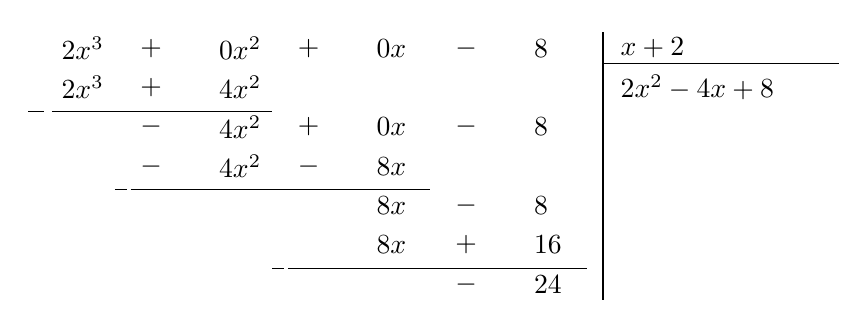
\begin{tikzpicture}
            \node[anchor=west] at (0,0) {\(2x^3\)};
            \node[anchor=west] at (1,0) {\(+\)};
            \node[anchor=west] at (2,0) {\(0x^2\)};
            \node[anchor=west] at (3,0) {\(+\)};
            \node[anchor=west] at (4,0) {\(0x\)};
            \node[anchor=west] at (5,0) {\(-\)};
            \node[anchor=west] at (6,0) {\(8\)};
            \node[anchor=west] at (0,-0.5) {\(2x^3\)};
            \node[anchor=west] at (1,-0.5) {\(+\)};
            \node[anchor=west] at (2,-0.5) {\(4x^2\)};
            \draw (0,-0.8) -- (2.8,-0.8);
            \draw (-0.3,-0.8) -- (-0.1,-0.8);
            \node[anchor=west] at (1,-1) {\(-\)};
            \node[anchor=west] at (2,-1) {\(4x^2\)};
            \node[anchor=west] at (3,-1) {\(+\)};
            \node[anchor=west] at (4,-1) {\(0x\)};
            \node[anchor=west] at (5,-1) {\(-\)};
            \node[anchor=west] at (6,-1) {\(8\)};
            \node[anchor=west] at (1,-1.5) {\(-\)};
            \node[anchor=west] at (2,-1.5) {\(4x^2\)};
            \node[anchor=west] at (3,-1.5) {\(-\)};
            \node[anchor=west] at (4,-1.5) {\(8x\)};
            \draw (1,-1.8) -- (4.8,-1.8);
            \draw (0.8,-1.8) -- (0.95,-1.8);
            \node[anchor=west] at (4,-2) {\(8x\)};
            \node[anchor=west] at (5,-2) {\(-\)};
            \node[anchor=west] at (6,-2) {\(8\)};
            \node[anchor=west] at (4,-2.5) {\(8x\)};
            \node[anchor=west] at (5,-2.5) {\(+\)};
            \node[anchor=west] at (6,-2.5) {\(16\)};
            \draw (3,-2.8) -- (6.8,-2.8);
            \draw (2.8,-2.8) -- (2.95,-2.8);
            \node[anchor=west] at (5,-3) {\(-\)};
            \node[anchor=west] at (6,-3) {\(24\)};
            \draw (7,-0.2) -- (10,-0.2);
            \draw (7,0.2) -- (7,-3.2);
            \node[anchor=west] at (7.1,0) {\(x+2\)};
            \node[anchor=west] at (7.1,-0.5) {\(2x^2-4x+8\)};
        \end{tikzpicture}
    \end{image}
  
     Besluit: \(2x^3-8=(2x^2-4x+8)(x+2)-24\)
    \end{oplossing}
\end{example}
 
\begin{example} Deel \(-x^3+9x+2\) door \(x+4\).
    \begin{oplossing}[toon] \nl
        \begin{image}[\width]
        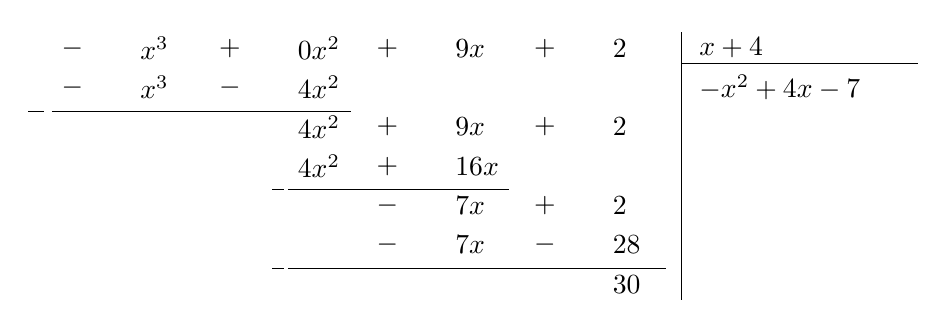
\begin{tikzpicture}
        \node[anchor=west] at (0,0) {\(-\)};
        \node[anchor=west] at (1,0) {\(x^3\)};
        \node[anchor=west] at (2,0) {\(+\)};
        \node[anchor=west] at (3,0) {\(0x^2\)};
        \node[anchor=west] at (4,0) {\(+\)};
        \node[anchor=west] at (5,0) {\(9x\)};
        \node[anchor=west] at (6,0) {\(+\)};
        \node[anchor=west] at (7,0) {\(2\)};
        \node[anchor=west] at (0,-0.5) {\(-\)};
        \node[anchor=west] at (1,-0.5) {\(x^3\)};
        \node[anchor=west] at (2,-0.5) {\(-\)};
        \node[anchor=west] at (3,-0.5) {\(4x^2\)};
        \draw (0,-0.8) -- (3.8,-0.8);
        \draw (-0.3,-0.8) -- (-0.1,-0.8);
        \node[anchor=west] at (3,-1) {\(4x^2\)};
        \node[anchor=west] at (4,-1) {\(+\)};
        \node[anchor=west] at (5,-1) {\(9x\)};
        \node[anchor=west] at (6,-1) {\(+\)};
        \node[anchor=west] at (7,-1) {\(2\)};
        \node[anchor=west] at (3,-1.5) {\(4x^2\)};
        \node[anchor=west] at (4,-1.5) {\(+\)};
        \node[anchor=west] at (5,-1.5) {\(16x\)};
        \draw (3,-1.8) -- (5.8,-1.8);
        \draw (2.8,-1.8) -- (2.95,-1.8);
        \node[anchor=west] at (4,-2) {\(-\)};
        \node[anchor=west] at (5,-2) {\(7x\)};
        \node[anchor=west] at (6,-2) {\(+\)};
        \node[anchor=west] at (7,-2) {\(2\)};
        \node[anchor=west] at (4,-2.5) {\(-\)};
        \node[anchor=west] at (5,-2.5) {\(7x\)};
        \node[anchor=west] at (6,-2.5) {\(-\)};
        \node[anchor=west] at (7,-2.5) {\(28\)};
        \draw (3,-2.8) -- (7.8,-2.8);
        \draw (2.8,-2.8) -- (2.95,-2.8);
        \node[anchor=west] at (7,-3) {\(30\)};
        \draw (8,-0.2) -- (11,-0.2);
        \draw (8,0.2) -- (8,-3.2);
        \node[anchor=west] at (8.1,0) {\(x+4\)};
        \node[anchor=west] at (8.1,-0.5) {\(-x^2+4x-7\)};
        \end{tikzpicture}
    \end{image}
 
    Besluit: \(-x^3+9x+2=(-x^2+4x-7)(x+4)+30\)
    \end{oplossing}
\end{example}
 
% Mmm, misschien beter een voorbeeld zonder breuken, en breuken laten tot in de oefeningen?
\begin{example} Deel \(4x^4+x^3+2x+1\) door \(2x^2+1\).
    \begin{oplossing}[toon] \nl
        \begin{image}[\width]
            \begin{tikzpicture}
            \node[anchor=west] at (0,0) {\(4x^4\)};
            \node[anchor=west] at (1,0) {\(+\)};
            \node[anchor=west] at (2,0) {\(x^3\)};
            \node[anchor=west] at (3,0) {\(+\)};
            \node[anchor=west] at (4,0) {\(0x^2\)};
            \node[anchor=west] at (5,0) {\(+\)};
            \node[anchor=west] at (6,0) {\(2x\)};
            \node[anchor=west] at (7,0) {\(+\)};
            \node[anchor=west] at (8,0) {\(1\)};
            \node[anchor=west] at (0,-0.5) {\(4x^4\)};
            \node[anchor=west] at (3,-0.5) {\(+\)};
            \node[anchor=west] at (4,-0.5) {\(2x^2\)};
            \draw (0,-0.8) -- (4.8,-0.8);
            \draw (-0.3,-0.8) -- (-0.1,-0.8);
            \node[anchor=west] at (2,-1) {\(x^3\)};
            \node[anchor=west] at (3,-1) {\(-\)};
            \node[anchor=west] at (4,-1) {\(2x^2\)};
            \node[anchor=west] at (5,-1) {\(+\)};
            \node[anchor=west] at (6,-1) {\(2x\)};
            \node[anchor=west] at (7,-1) {\(+\)};
            \node[anchor=west] at (8,-1) {\(1\)};
            \node[anchor=west] at (2,-1.5) {\(x^3\)};
            \node[anchor=west] at (5,-1.5) {\(+\)};
            \node[anchor=west] at (6,-1.5) {\(\tfrac12 x\)};
            \draw (2,-1.8) -- (6.8,-1.8);
            \draw (1.8,-1.8) -- (1.95,-1.8);
            \node[anchor=west] at (3,-2) {\(-\)};
            \node[anchor=west] at (4,-2) {\(2x^2\)};
            \node[anchor=west] at (5,-2) {\(+\)};
            \node[anchor=west] at (6,-2) {\(\tfrac32 x\)};
            \node[anchor=west] at (7,-2) {\(+\)};
            \node[anchor=west] at (8,-2) {\(1\)};
            \node[anchor=west] at (3,-2.5) {\(-\)};
            \node[anchor=west] at (4,-2.5) {\(2x^2\)};
            \node[anchor=west] at (7,-2.5) {\(-\)};
            \node[anchor=west] at (8,-2.5) {\(1\)};
            \draw (3,-2.8) -- (8.8,-2.8);
            \draw (2.8,-2.8) -- (2.95,-2.8);
            \node[anchor=west] at (6,-3) {\(\tfrac32 x\)};
            \node[anchor=west] at (7,-3) {\(+\)};
            \node[anchor=west] at (8,-3) {\(2\)};
            \draw (9,-0.2) -- (12,-0.2);
            \draw (9,0.2) -- (9,-3.2);
            \node[anchor=west] at (9.1,0) {\(2x^2+1\)};
            \node[anchor=west] at (9.1,-0.5) {\(2x^2+\tfrac12 x-1\)};
            \end{tikzpicture}
        \end{image}
    Besluit: \(4x^4+x^3+2x+1= \left(2x^2+\frac{1}{2}x-1\right)(2x^2+1)+\left(\frac{3}{2}x+2\right)\)
    \end{oplossing}
\end{example}



\end{document}
